%	PACKAGES AND OTHER DOCUMENT CONFIGURATIONS

\documentclass[11pt, a4paper]{article} % 10pt font size (11 and 12 also possible), A4 paper (letterpaper for US letter) and two column layout (remove for one column) Use additional titlepage argument to generate this
%\documentclass[12pt, a4paper,twocolumn,titlepage]{article}

%%%%%%%%%%%%%%%%%%%%%%%%%%%%%%%%%%%%%%%%%
% Wenneker Article
% Structure Specification File
% Version 1.0 (28/2/17)
%
% This file originates from:
% http://www.LaTeXTemplates.com
%
% Authors:
% Frits Wenneker
% Vel (vel@LaTeXTemplates.com)
%
% License:
% CC BY-NC-SA 3.0 (http://creativecommons.org/licenses/by-nc-sa/3.0/)
%
%%%%%%%%%%%%%%%%%%%%%%%%%%%%%%%%%%%%%%%%%

%----------------------------------------------------------------------------------------
%	PACKAGES AND OTHER DOCUMENT CONFIGURATIONS
%----------------------------------------------------------------------------------------

\usepackage[english]{babel} % English language hyphenation

\usepackage{microtype} % Better typography

\usepackage{verbatim} % Allows mulitline commenting

\usepackage{amsmath,amsfonts,amsthm} % Math packages for equations

\usepackage[svgnames]{xcolor} % Enabling colors by their 'svgnames'

\usepackage[hang, small, labelfont=bf, up, textfont=it]{caption} % Custom captions under/above tables and figures

\usepackage{subcaption}

\usepackage{booktabs} % Horizontal rules in tables

\usepackage{lastpage} % Used to determine the number of pages in the document (for "Page X of Total")

\usepackage{graphicx} % Required for adding images

\usepackage{enumitem} % Required for customising lists
\setlist{noitemsep} % Remove spacing between bullet/numbered list elements

\usepackage{sectsty} % Enables custom section titles
\allsectionsfont{\usefont{OT1}{phv}{b}{n}} % Change the font of all section commands (Helvetica)

\usepackage{siunitx}

%----------------------------------------------------------------------------------------
%	MARGINS AND SPACING
%----------------------------------------------------------------------------------------

\usepackage{geometry} % Required for adjusting page dimensions

\geometry{
	top=1cm, % Top margin
	bottom=1.5cm, % Bottom margin
	left=2cm, % Left margin
	right=2cm, % Right margin
	includehead, % Include space for a header
	includefoot, % Include space for a footer
	%showframe, % Uncomment to show how the type block is set on the page
}

\setlength{\columnsep}{7mm} % Column separation width

%----------------------------------------------------------------------------------------
%	FONTS
%----------------------------------------------------------------------------------------

\usepackage[T1]{fontenc} % Output font encoding for international characters
\usepackage[utf8]{inputenc} % Required for inputting international characters

\usepackage{XCharter} % Use the XCharter font

%----------------------------------------------------------------------------------------
%	HEADERS AND FOOTERS
%----------------------------------------------------------------------------------------

\usepackage{fancyhdr} % Needed to define custom headers/footers
\pagestyle{fancy} % Enables the custom headers/footers

\renewcommand{\headrulewidth}{0.0pt} % No header rule
\renewcommand{\footrulewidth}{0.4pt} % Thin footer rule

\renewcommand{\sectionmark}[1]{\markboth{#1}{}} % Removes the section number from the header when \leftmark is used

%\nouppercase\leftmark % Add this to one of the lines below if you want a section title in the header/footer

% Headers
\lhead{} % Left header
\chead{\textit{\thetitle}} % Center header - currently printing the article title
\rhead{} % Right header

% Footers
\lfoot{} % Left footer
\cfoot{} % Center footer
\rfoot{\footnotesize Page \thepage\ of \pageref{LastPage}} % Right footer, "Page 1 of 2"

\fancypagestyle{firstpage}{ % Page style for the first page with the title
	\fancyhf{}
	\renewcommand{\footrulewidth}{0pt} % Suppress footer rule
}

%----------------------------------------------------------------------------------------
%	TITLE SECTION
%----------------------------------------------------------------------------------------

\newcommand{\authorstyle}[1]{{\large\usefont{OT1}{phv}{b}{n}\color{NavyBlue}#1}} % Authors style (Helvetica)

\newcommand{\institution}[1]{{\footnotesize\usefont{OT1}{phv}{m}{sl}\color{Black}#1}} % Institutions style (Helvetica)

\usepackage{titling} % Allows custom title configuration

\newcommand{\HorRule}{\color{SteelBlue}\rule{\linewidth}{1pt}} % Defines the gold horizontal rule around the title

\pretitle{
	\vspace{-30pt} % Move the entire title section up
	\HorRule\vspace{10pt} % Horizontal rule before the title
	\fontsize{32}{36}\usefont{OT1}{phv}{b}{n}\selectfont % Helvetica
	\color{Navy} % Text colour for the title and author(s)
}

\posttitle{\par\vskip 15pt} % Whitespace under the title

\preauthor{} % Anything that will appear before \author is printed

\postauthor{ % Anything that will appear after \author is printed
	\vspace{10pt} % Space before the rule
	\par\HorRule % Horizontal rule after the title
	\vspace{20pt} % Space after the title section
}

%----------------------------------------------------------------------------------------
%	ABSTRACT
%----------------------------------------------------------------------------------------

\usepackage{lettrine} % Package to accentuate the first letter of the text (lettrine)
\usepackage{fix-cm}	% Fixes the height of the lettrine

\newcommand{\initial}[1]{ % Defines the command and style for the lettrine
	\lettrine[lines=3,findent=4pt,nindent=0pt]{% Lettrine takes up 3 lines, the text to the right of it is indented 4pt and further indenting of lines 2+ is stopped
		\color{NavyBlue}% Lettrine colour gold DarkGoldenRod
		{#1}% The letter
	}{}%
}

\usepackage{xstring} % Required for string manipulation

\newcommand{\lettrineabstract}[1]{
	\StrLeft{#1}{1}[\firstletter] % Capture the first letter of the abstract for the lettrine
	\initial{\firstletter}\textbf{\StrGobbleLeft{#1}{1}} % Print the abstract with the first letter as a lettrine and the rest in bold
}

%	BIBLIOGRAPHY

\usepackage[backend=biber,style=phys,natbib=true,doi=false]{biblatex} 
%Can equally use numeric citation style without extra phys packaging (but doesn't change capitalisation), or authoryear for alphabetical listing without the codes (resembles APA)

%\addbibresource{references.bib} % The filename of the bibliography

\usepackage[autostyle=true]{csquotes} % Required to generate language-dependent quotes in the bibliography

%    APPENDICES

\usepackage[title]{appendix} %in appendix


 % Specifies the document structure and loads requires packages
\graphicspath{{"/Users/kit gallagher/Documents/Research Review/Report/Figures"}}
\newcommand*{\subscript}[1]{\ensuremath{_\textrm{{\scriptsize #1}}}}

%	ARTICLE INFORMATION

\title{Simulating Liquid Crystals}

%\author{
	%\authorstyle{Christopher Gallagher}}
\author{\authorstyle{Kit Gallagher} 
	%\institution{University of Cambridge \\
	\institution{Supervisors: Prof Erika Eiser, Mr Jiaming Yu}}
% Example of a one line author/institution relationship
%\author{\newauthor{John Marston} \newinstitution{Universidad Nacional Autónoma de México, Mexico City, Mexico}}

\date{\today} % Add a date here if you would like one to appear underneath the title block, use \today for the current date, leave empty for no date
\usepackage[english]{babel}
\usepackage{tabularx}
%\renewcommand{\thefootnote}{\roman{footnote}}  %use roman lettering for footnotes instead
%\usepackage[backend=biber,doi=false]{biblatex}
\addbibresource{reportreferences.bib}
%\AtBeginBibliography{\small}
%----------------------------------------------------------------------------------------
\begin{document}
	
%Your project should contain the following statement on the first page of the project: Except where specific reference is made to the work of others, this work is original and has not been already submitted either wholly or in part to satisfy any degree requirement at this or any other university.	A link to your on-line notebook should also be added to the first page of your report before uploading the project.

\maketitle % Print the title

\thispagestyle{firstpage} % Apply the page style for the first page (no headers and footers)

%	ABSTRACT

\lettrineabstract{The specificity of DNA base-pair interactions gives considerable functional control in the design of anisotropic nano-particles, enabling the formation of liquid crystal phases. This project aims to study the liquid phase behaviour of such non-conventional liquid crystal molecules, with a particular focus on the novel `nunchuck' structure - two rigid rods connected via a flexible linker. The Eiser Group have previously considered intra-molecular interaction potentials at the single-nucleotide level for a single DNA nanoparticle, and I am now implementing these potentials in larger, more coarse-grained models of multiple nanoparticles, through open-source software LAMMPS (Large-scale Atomic/Molecular Massively Parallel Simulator). Such systems are expected to form smectic (layered) phases at high volume fractions. THIS WILL BE EDITED AT THE END}

\section{Introduction}
What are we studying? (brief)
Why are we interested? Applications of this!

Outline of report

\section{Background}
\subsection{Liquid Crystals}
Include known phases etc 
\subsection{Onsager Theory}
Introduce theoretical predictions to be validated later
Mathematical derivations may be provided in appendicies
\subsection{Previous Computational Work} \label{sec:PrevWork}

\section{Methods}
As introduced in Section \ref{sec:PrevWork}, all molecular dynamics simulations were completed in LAMMPS. LAMMPS (Large-scale Atomic/Molecular Massively Parallel Simulator) is a medium coarse-grained, classical molecular dynamics code developed to replicate  solid-state materials and soft matter mesoscopic systems \cite{Plimpton1995, LAMMPS}.


%Can expand on this if needs be, from rapaport

\subsection{Simulation Molecules}
As introduced in Section \textbf{X}, we are considering `nunchuck' molecules formed of two rigid rods connected by a flexible linker, as depicted in Figure \ref{fig:nunchuck_analogy}. However, as the interaction potential of an anisotropic particle is rather complex, it is computationally simpler to consider each molecule as a system of connected spheres, each with a separate isotropic interaction potential (detailed further in Section \ref{pair_potential}).

This is visualised in Figure \ref{fig:nunchuck_implementation}, for rigid rods of aspect ratio 7. The ss-DNA is represented by a further sphere in the centre of the molecule, coloured differently in red to highlight its differing mechanical properties. It has a modified bond angle, so the molecule is bent around this element, and reduced bond rigidity so the particle may also stretch about this point.



\begin{figure}[ht]
	\hfill  %NOT SURE ABOUT THIS!
	\begin{subfigure}{.4\textwidth}
		\centering
		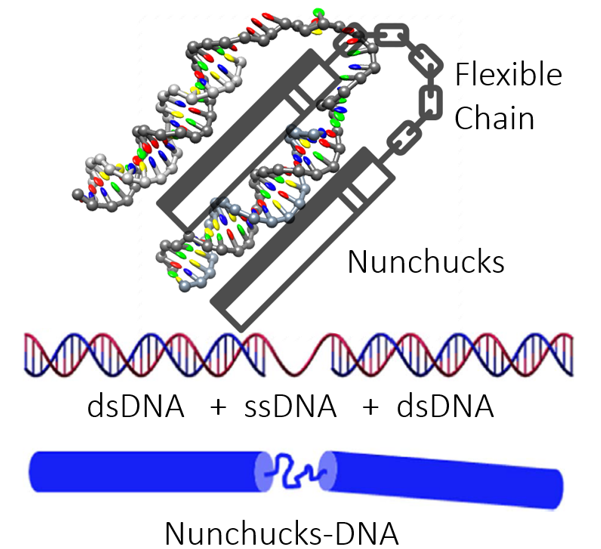
\includegraphics[width=\linewidth]{Figures/nunchucks_artist}  
		\caption{Coarse-grained Model}
		\label{fig:nunchuck_analogy}
	\end{subfigure}
	\hfill %% useful if width of each figure is less the .5\textwidth
	\begin{subfigure}{.4\textwidth}
		\centering
		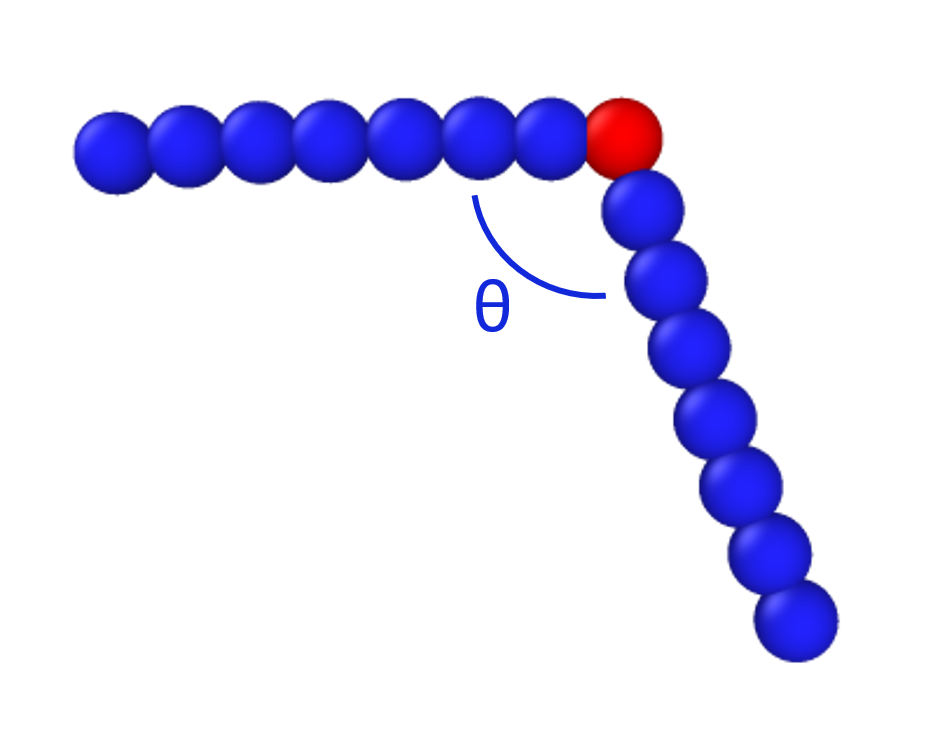
\includegraphics[width=\linewidth]{Figures/nunchuck_profile_coloured}  
		\caption{LAMMPS Implementation}
		\label{fig:nunchuck_implementation}
	\end{subfigure}
	\caption{Depiction analogy between the DNA mesogen and the nunchucks. Note the appearance of the flexible ss-DNA linker between the rigid ds-DNA rods, and the implementation within LAMMPS on the right. The central red sphere, representing the ss-DNA, is given modified bond properties to replicate the nunchuck's flexibility. Figure (a) created by Jiaming Yu (Eiser Group, Cambridge).}
	\label{fig:nunchucks_visual}
	\hfill
\end{figure}

The nunchucks are formed of two rigid rods of ds-DNA, connected via a flexible linker of ss-DNA, and the complete nunchuck is modelled as a rod of 60 base pairs long. With the standard values for DNA of radius $r = 2$nm and length (per base pair) of $l=0.33$nm, we obtain an aspect ratio of 10 for this rod. . Within LAMMPS, this is expressed as ten spherical balls (aspect ratio 1) bound rigidly together in a linear structure. 

It should be noted that a system of natural units is used throughout this paper. Based on the Lennard-Jones potential, the cut-off length and characteristic energy are both set to unity. The simulation timescale is then fixed by the choice of these values, and the mass of the simulation body. 

The physical values for a system may be considered for a specific system (in this case strands of ds-DNA) through scaling via the relevant mass, length scale and energy scale of this system. However the dimensionless simulations presented here may be applied to any similarly-shaped mesogens; we would expect other systems to display the same behaviour over a timescale determined by their material properties \cite{Rapaport2004}.

For the nunchuck particles considered, a lengthscale of 2nm corresponds to particle size.

It is worth noting that the persistence length of DNA is around 50nm \cite{Garcia2007}, so the approximation of perfect rigidity is valid over the length-scale of the molecule.

\subsection{Intermolecular Potential} \label{pair_potential}
parameters and potentials used etc.
Timescales and simulation sizes used etc


A shifted, cut-off Lennard-Jones potential was chosen to represent pair-wise interactions between molecules. While the Lennard-Jones potential \cite{Jones1924a, Jones1924b} has long been the natural choice for molecular dynamics simulations \cite{Stephan2019}, its infinite range introduces computational complexity as interactions between all pairs of particles must be considered. It is therefore increasingly common to use a cut-off version, whereby the potential is set to zero beyond a `cut-off' radius, and here we chose to neglect the entire attractive tail. As well as simplifying the calculations required, this also allows our results to be generalised to any mesogens without attractive inter-molecular forces (that typically favour ordered-phase formation), as any phase transitions observed here must be purely entropically driven. This is commonly known as a soft-core model, where particle overlap is suppressed via this repulsive potential rather than any excluded volume interactions, and is computationally much less demanding \cite{Paolini1993, Hughes2008}.
%can cite frenkel on entropically drive transitions if req

However, this cut-off may cause unphysical behaviour if the potential does not tend to zero smoothly at this point. This is remedied by the addition of a constant term, described in the full form of the pair-wise potential $U_{ij}$ in (\ref{lj_cut}):

\begin{equation} \label{lj_cut}
U_{ij} = 4\epsilon \left[ \left( \frac{\sigma}{r_{ij}} \right) ^{12} - \left( \frac{\sigma}{r_{ij}} \right) ^{6}	\right] + \epsilon \qquad	 r_{ij} < r_{c} = 2^{1/6} \sigma
\end{equation}

Here $\sigma$ and $\epsilon$ are the relevant length and energy scales of the system, formally corresponding to the particle separation at which the $U_{ij} = 0$, and the depth of the potential well. It is worth noting that the effects of this truncation and shift on the overall thermodynamic quantities are well documented \cite{Stephan2020, Shaul2010}, and changes in lyotropic properties are negligible in 3D bulk liquids with a conserved particle number \cite{Smit1991}. 


 
\subsection{Analysis}
Includes custom written python scripts and OVITO freeware. Credit scripts written by other group members.

\section{Rigid Rod Simulations}


\section{Nunchuck Simulations}



\section{Conclusion}
Summarise key results from above, and emphasise their importance 
Also give limitations of results obtained, and suggest direction for further work


%\clearpage
\printbibliography

\begin{appendices}

\section{Onsager Theory}
\section{Netamtic Order Parameter}
include theoretical derivation and calculation

\section{Code?}

\end{appendices}

\end{document}


%%%%%%%%%%%%%%%%%%%%%%%%%%%%%%%%%%%%%%%%%
% Wenneker Article
% LaTeX Template
% Version 2.0 (28/2/17)
%
% This template was downloaded from:
% http://www.LaTeXTemplates.com
%
% Authors:
% Vel (vel@LaTeXTemplates.com)
% Frits Wenneker
%
% License:
% CC BY-NC-SA 3.0 (http://creativecommons.org/licenses/by-nc-sa/3.0/)
%
%%%%%%%%%%%%%%%%%%%%%%%%%%%%%%%%%%%%%%%%%
